\section{Ахова працы}

\subsection{Арганізацыя сістэмы кіравання аховай працы на прадпрыемстве}

Сістэма кіравання аховай працы (АП) у замежным таварыстве з абмежаванай адказнасцю «ЭПАМ Сістэмз», прызначана для прадухілення траўм і захворванняў, звязаных з вытворчай дзейнасцю, а таксама для абароны і ўмацавання здароўя супрацоўнікаў арганізацыі; яна таксама накіравана на паляпшэнне ўмоў працы і навакольнага асяроддзя.

На малюнку \ref{img: epam healthy system} прадстаўлена структура службы аховы працы ў арганізацыі «ЭПАМ Сістэмз».

\begin{figure}[h!]
    \centering
    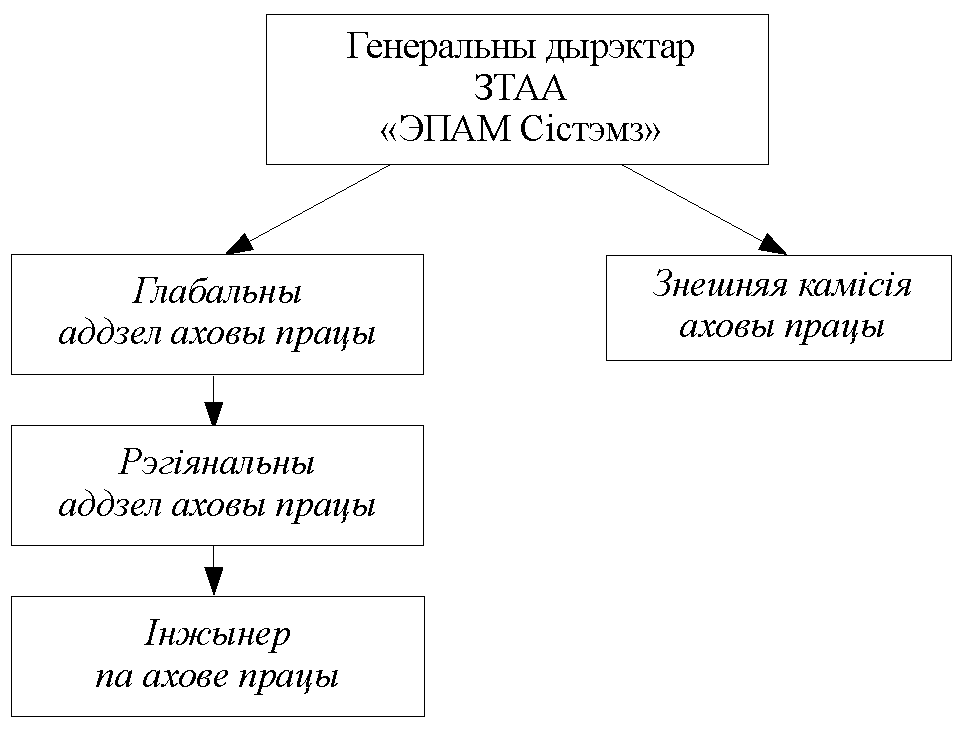
\includegraphics[width=0.7\textwidth]{epam_healthy_system.pdf}
    \caption{Структура службы аховы працы ў арганізацыі}
    \label{img: epam healthy system} 
\end{figure}

Штогод, у мэтах далейшага ўдасканалення арганізацыі работ па АП і забеспячэння выканання заканадаўства аб АП, генеральны дырэктар сцвярджае план мерапрыемстваў, складзены дырэктарам адміністрацыйнага дэпартамента і начальнікам глабальнага аддзела АП, якi ўключае:
\begin{enumerate}
    \item удасканаленне дакументацыі па АП, неабходнай у арганізацыі, ўкараненне перадавога досведу і навуковых распрацовак па АП і ТБ у арганізацыі;
    \item правядзенне папярэдніх медыцынскіх аглядаў, кансультацыі з дактарамі вузкіх спецыялізацый і вакцынацыя супрацоўнікаў перад прагназуемымі перыядамі эпідэміялагічных захворванняў;
    \item набыццё мыйных сродкаў і сродкаў асабістай гігіены для супрацоўнікаў арганізацыі, закупка сродкаў індывідуальнай абароны;
    \item арганізацыя правядзення лабараторна-інструментальных даследаванняў фактараў вытворчага асяроддзя на працоўных месцах у арандаваных памяшканнях;
    \item ажыццяўленне кантролю за правядзеннем перыядычных (паўторных) інструктажоў па АП і пажарнай бяспекі (ПБ) у вытворчых падраздзяленнях арганізацыі;
    \item выяўленне вытворчых небяспекі з мэтай кіравання (зніжэння) рызык перадумоў стварэння сітуацый, якія прыводзяць да няшчасных выпадкаў;
    \item забеспячэнне тэхнічна абгрунтаваных умоў эксплуатацыі сістэм вентыляцыі і кандыцыянавання, а таксама абследаванне і кантроль за станам апорных канструкцый будынкаў.
\end{enumerate}

Кіраўнікі дэпартаментаў арганізацыі павінны быць азнаёмлены з загадам аб зацвярджэнні плана мерапрыемстваў па АП, пры гэтым кантроль за выкананнем загаду ускладаецца на дырэктара адміністрацыйнага дэпартамента.

Чаканая сацыяльная эфектыўнасць ад увядзення мерапрыемстваў па АП:
\begin{enumerate}
    \item зніжэнне імавернасці ўзнікнення траўманебяспечных сiтуацый;
    \item падтрыманне умоў працы на працоўных месцах арганізацыі ў адпаведнасці з санітарна-гігіенічнымі нормамі;
    \item паляпшэнне ўмоў навучання, правядзення інструктажоў у арганізацыі;
    \item фарміраванне нарматыўнай базы ў арганізацыі;
    \item зніжэнне рызык ўзнікнення агульных захворванняў;
    \item маніторынг умоў працы на працоўных месцах арганізацыі.
\end{enumerate}

Інжынер па ахове працы, у адпаведнасці са сваімі паўнамоцтвамі, мае права:
\begin{enumerate}
    \item праводзіць праверкі выканання патрабаванняў па АП, стану ўмоў працы;
    \item запытваць і атрымліваць неабходную інфармацыю па пытаннях АП, патрабаваць пісьмовыя тлумачэнні ад службовых асоб, якія працуюць і якія дапусцілі парушэнні патрабаванняў па АП;
    \item прыпыняць ва ўстаноўленым заканадаўствам парадку эксплуатацыю абсталявання, інструмента, прыстасаванняў, транспартных сродкаў, выкананне работ (аказанне паслуг) пры выяўленні парушэнняў, якія ствараюць пагрозу для жыцця або здароўя супрацоўнікаў і навакольных, да іх ліквідацыі;
    \item уносіць прапановы па паляпшэнню ўмоў працы супрацоўнікаў, папярэджваючы вытворчы траўматызм і прафесійныя захворванні.
\end{enumerate}

Такім чынам, асноўнымі задачамі службы аховы працы ў арганізацыі з'яўляюцца:
\begin{enumerate}
    \item арганізацыя навучання і праверкі ведаў супрацоўнікаў па пытаннях аховы працы;
    \item арганізацыя і каардынацыя мерапрыемстваў па ахове працы ў арганізацыі;
    \item кантроль за выкананнем патрабаванняў па АП;
    \item удасканаленне ўмоў працы і правядзенне прафілактычных работ па папярэджанні вытворчага траўматызму, прафесійных і вытворча абумоўленых захворванняў.
\end{enumerate}

\subsection{Ідэнтыфікацыя і аналіз шкодных і небяспечных фактараў}

Арганізацыя «ЭПАМ Сістэмз» валодае мноствам структурных падраздзяленняў, сярод якіх: некалькі дэпартаментаў па распрацоўцы праграмнага забеспячэння, дэпартамент па інфармацыйным забеспячэнні, аддзяленне развіцця сeрвісаў, адміністрацыйны дэпартамент, аддзяленне кіравання персаналам, тэхнічнае аддзяленне, фінансавы дэпартамент і іншыя.

У дадзеным раздзеле будзе праведзена ідэнтыфікацыя шкодных і небяспечных вытворчых фактараў для дэпартамента па распрацоўцы праграмнага забеспячэння.

Дадзены дэпартамент быў абраны, так як распрацоўка праграмнага забеспячэння
з'яўляецца галоўнай функцыяй арганізацыі, а значыць большая частка супрацоўнікаў належыць да дазенага дэпартамента.

Шкодны вытворчы фактар --- гэта фактар, які можа прывесці да розных захворванняў або пагоршыць ўжо існуючыя захворванні.

Небяспечны вытворчы фактар --- гэта фактар, які можа прывесці да траўмы, у тым ліку смяротнай.

Класіфікацыя небяспечных і шкодных вытворчых фактараў па прыродзе ўплыву на здароўе чалавека падрадзяляюцца на:
\begin{enumerate}
    \item фізічныя;
    \item хімічныя;
    \item біялагічныя;
    \item псіхафізіалагічныя.
\end{enumerate}

Наяўнасць фізічных фактараў галоўным чынам абумоўлена выкананнем работ на персанальным камп'ютары пры стварэнні праграмнага забеспячэння. Фізічныя фактары пры працы за камп'ютарам: павышаны ўзровень электрамагнітных выпраменьванняў, падвышаная напружанасць электрычнага поля, падвышанае значэнне напругі ў электрычным ланцугу, замыканне, павышаны ўзровень статычнай электрычнасці, адсутнасць або недахоп натуральнага святла, недастатковая штучная асветленасць працоўнай зоны, падвышаная яркасць святла, падвышаная кантраснасць, манатоннасць працоўнага працэсу.

Галоўным псіхалагічным фактарам у дэпартаменце па распрацоўцы праграмнага забеспячэння з'яўляецца разумовае напружанне, якое можа быць выклікана манатоннасцю працы, невыкананнем рэжыму працы і адпачынку, пастаянная высокая канцэнтрацыя ўвагі, эмацыйная і псіхалагічная нагрузка.

У дэпартаменце па распрацоўцы праграмнага забеспячэння адсутнічаюць непаспрэдныя хімічныя і біялагічныя шкодныя і небяспечныя вытворчыя фактары,
аднак у дэпартаменце па распрацоўцы праграмнага забеспячэння могуць
з'явіцца другасныя біялагічныя шкодныя і небяспечныя фактары (напрыклад, пандэмія інфекцыі COVID-19).

\subsection{Арганізацыйныя, тэхналагічныя і іншыя рашэнні для
ўстаранення небяспечных і шкодных фактараў}

Небяспечныя і шкодныя вытворчыя фактары становяцца такімі і прыводзяць да парушэння здароўя спецыялістаў, калі іх велічыні перавышаюць гранічна дапушчальныя велічыні, зацверджаныя ва ўстаноўленым парадку.

Згодна з пунктам 8 санітарных норм і правілаў «Гігіенічная класіфікацыя ўмоў працы», зацверджаных пастановай Міністэрства аховы здароўя РБ ад 2012/12/28 № 211, умовы працы дзеляцца на 4 класы:
\begin{enumerate}
    \item 1 клас --- аптымальныя ўмовы працы;
    \item 2 клас --- дапушчальныя ўмовы працы;
    \item 3 клас --- шкодныя ўмовы працы;
    \item 4 клас --- небяспечныя ўмовы працы.
\end{enumerate}

У табліцах \ref{table: healthy1} і \ref{table: healthy2} прыведзены гранічна дапушчальныя ўзроўні электрамагнітных палёў ад ВДТ, ЭВМ і перыферыйных прылад у адпаведнасці з гігіенічным нарматывам «Гранічна дапушчальныя ўзроўні нарміруемых параметраў пры працы з відэадысплейнымі тэрміналамі і электронна-вылічальнымі машынамі».

\begin{table}[htp]
    \caption{Гранічна дапушчальныя ўзроўні электрамагнітных палёў ад ВДТ і ЭВМ}
    \begin{tabularx}{\textwidth}{ | >{\centering\arraybackslash}X
                                  | >{\centering\arraybackslash}X | }
    \hline
        Назва параметра & Гранічна дапушчальныя ўзроўні \\
    \hline
        Напрыжанасць электрычнага поля
        ў дыяпазоне частот & \\
    \hline
        5 Гц - 2 кГц & Не больш за 25 В/м \\
    \hline
        2-400 кГц & Не больш за 2,5 В/м \\
    \hline
        Шчыльнасць магнітнага патоку магнітнага поля
        ў дыяпазоне частот & \\
    \hline
        5 Гц - 2 кГц & Не больш за 250 нТл \\
    \hline
        2-400 кГц & Не больш за 25 нТл \\
    \hline
        Напружанасць электрастатычнага поля & Не больш за 15 кВ/м \\
    \hline
    \end{tabularx}
    \label{table: healthy1}
\end{table}

\vspace{-\baselineskip}

\begin{table}[htp]
    \caption{Гранічна дапушчальныя ўзроўні электрамагнітных палёў ад перыферыйных прылад}
    \begin{tabularx}{\textwidth}{ | >{\centering\arraybackslash}X
                                  | >{\centering\arraybackslash}X
                                  | >{\centering\arraybackslash}X
                                  | >{\centering\arraybackslash}X
                                  | >{\centering\arraybackslash}X
                                  | >{\centering\arraybackslash}X | }
    \hline
        Дыяпазон частот & 0,3 - 300 кГц &
        0,3 - 3 МГц & 3 - 30 МГц & 30 - 300 МГц & 0,3 - 300 ГГц\\
    \hline
        Гранічна дапушчальныя ўзроўні & 25 В/м &
        15 В/м & 10 В/м & 3 В/м & 10 мкВт/кв. см \\
    \hline
    \end{tabularx}
    \label{table: healthy2}
\end{table}

У табліцы \ref{table: healthy3} прыведзены гранічна дапушчальныя ўзроўні інтэнсіўнасці выпраменьвання з боку экрана ВДТ і ЭВМ. У табліцы
\ref{table: healthy4} прыведзены дапушчальныя візуальныя эрганамічныя параметры прылад адлюстравання ВДТ і ЭВМ.

\begin{table}[htp]
    \caption{Гранічна дапушчальныя ўзроўні інтэнсіўнасці выпраменьвання
    з боку экранаў ВДТ і ЭВМ}
    \begin{tabularx}{\textwidth}{ | >{\centering\arraybackslash}X
                                  | >{\centering\arraybackslash}X
                                  | >{\centering\arraybackslash}X
                                  | >{\centering\arraybackslash}X | }
    \hline
        Дыяпазон даўжыні хваль & 200 - 280 нм &
        280 - 315 нм & 315 - 400 нм \\
    \hline
        Гранічна дапушчальныя ўзроўні & Не дапушчальны &
        0,0001 Вт/кв. м. & 0,1 Вт/кв. м. \\
    \hline
    \end{tabularx}
    \label{table: healthy3}
\end{table}

\clearpage

\begin{table}[htp]
    \caption{Дапушчальныя візуальныя эрганамічныя параметры прылад
    адлюстравання ВДТ і ЭВМ}
    \begin{tabularx}{\textwidth}{ | >{\centering\arraybackslash}X
                                  | >{\centering\arraybackslash}X | }
    \hline
        Параметры & Дапушчальныя значэнні \\
    \hline
        Яркасць белага поля & Не менш за 35 кд/кв. м \\
    \hline
        Нераўнамернасць яркасці працоўнага поля & Не больш за +/-20\% \\
    \hline
         Кантрастнасць (манахромны рэжым) & Не менш за 3:1 \\
    \hline
        Часавая нестабільнасць выявы & Не павінна фіксавацца \\
    \hline
        Частата абнаўлення выявы (дыскрэтны экран) & Не менш за 60 Гц \\
    \hline
    \end{tabularx}
    \label{table: healthy4}
\end{table}

У арганізацыі <<ЭПАМ Сістэмз>> для падтрымкі аховы працы дзейнічае
дакумент аб ахове здароўя (EPAM Health and Safety Framework), якога павінны пільнавацца
ўсе супрацоўнікі арганізацыі.

Элементы аховы здароўя ЭПАМ Сістэмз забяспечваюць:
\begin{enumerate}
    \item маніторынг заканадаўства і нормаў, звязаных з EHS, і выкананне ўсіх дзеючых патрабаванняў;
    \item бяспечнае і здаровае працоўнае асяроддзе для ўсіх супрацоўнікаў і падрадчыкаў, якое адпавядае нарматыўным патрабаванням і перадавой практыцы кіравання;
    \item устаноўленыя працэдуры распазнавання, ацэнкі і кантролю небяспекі для здароўя і бяспекі на аб'екце;
    \item Адэкватны ўзровень падрыхтоўкі спецыялістаў па ахове працы для ўсіх супрацоўнікаў і падрадчыкаў;
    \item ухіленне неабгрунтаваных рызык, звязаных з сродкамі, паслугамі і іншымі відамі работ;
    \item мінімізацыя выкарыстання і выкіду таксічных і небяспечных матэрыялаў;
    \item улік уздзеяння EHS пры распрацоўцы і вытворчасці паслуг ЭПАМ з мэтай паўторнага выкарыстання сыравіны і прадухілення забруджвання навакольнага асяроддзя;
    \item пастаянная ацэнка і абнаўленне праграм па ахове здароўя і бяспекі для забеспячэння пастаяннага ўдасканалення і даўгавечнай эфектыўнасці.
\end{enumerate}

Калі супрацоўнік не ведае, як выканаць пэўную задачу, альбо лічыць, што выкананне гэтай задачы альбо выкарыстанне абсталявання небяспечна, ён абавязаны як мага хутчэй паведаміць пра гэта свайму кіраўніку. Акрамя таго, супрацоўнік можа, калі захоча, спаслацца на працэдуру разгляду зваротаў ЭПАМ, альбо можа падаць скаргу ў адпаведнасці з палажэннямі ЭПАМ аб раскрыцці інфармацыі ў грамадскім інтарэсе.

Для прадухілення біялагічных фактараў уздзеяння на супрацоўнікаў быў распрацаваны план прадухілення і рэакцыі на масавыя захворванні.

На малюнку \ref{img: pandemic prevention} прадстаўлены асноўныя крокі для
прадухілення масавага захворвання.

\clearpage

\begin{figure}[ht!]
    \centering
    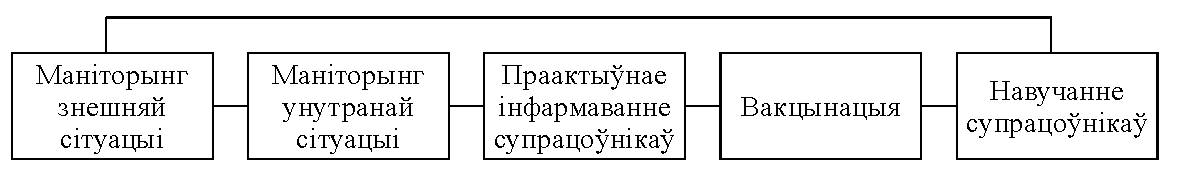
\includegraphics[width=\textwidth]{pandemic_prevention.pdf}
    \vspace{-1.4\baselineskip}
    \caption{План прадухілення масавага захворвання}
    \label{img: pandemic prevention}
\end{figure}

Коратка разгледзім крокі плана прадухілення масавага захворвання:
\begin{enumerate}
    \item маніторынг знешняй сітуацыі: начальнік вядзе спіс кантактаў медыцынскіх спецыялістаў, каб мець кансультацыю і параду адносна гэтага плана і яго рэалізацыі. Усе паведамленні пра любую пандэмічную пагрозу, якая можа выклікаць сур'ёзную распаўсюджаную хваробу, публікуюцца ў дзяржаўных сродках масавай інфармацыі;
    \item маніторынг унутранай сітуацыі: начальнік штотыдзень запытвае
    справаздачу пра ўнутраныя заяўкі на бальнічныя лісты і дні. Калі колькасць хворых супрацоўнікаў павялічыцца да 5\%, начальнік інфармуе кіраўнікоў рэсурсаў, кіраўнікоў уліковых запісаў і членаў групы па пандэмічных рэагаваннях па электроннай пошце пра статыстыку і дае далейшыя інструкцыі;
    \item праактыўнае інфармаванне супрацоўнікаў: начальнік таксама распрацаўвае спіс рэкамендаваных прэпаратаў для барацьбы з інфекцыямі для служб кіравання офісам (напрыклад, мыла, адмысловыя тканіны, маскі і дэзінфікуючыя сродкі). Адміністрацыйныя службы, якія адказваюць за кожнае месца, маюць дастатковую колькасць для іх пастаяннага абнаўлення.
    \item навучанне супрацоўнікаў: начальнік, прынамсі, штогод і перад сезонам вірусных захворванняў прадастаўляе інфармацыю ўсім супрацоўнікам адносна практыкі, рэкамендаванай службовымі асобамі аховы здароўя для зніжэння распаўсюджвання інфекцыі. Запрашаецца эпідэміёлаг на публічную лекцыю пра тое, як паводзіць сябе ў сезон віруснага захворвання і як рэагаваць у выпадку якіх-небудзь унікальных заразных/інфекцыйных захворванняў.
\end{enumerate}

\subsection{Эрганоміка}

Эрганоміка --- навуковая і практычная дысцыпліна, якая сфармавалася на стыку псіхалогіі, фізіялогіі, гігіены працы, біямеханікі, антрапалогіі і шэрагу тэхнічных навук. Міждысцыплінарнае вывучэнне чалавека ці групы людзей ва ўмовах іх дзейнасці з прымяненнем тэхнічных сродкаў складае сутнасць эрганомікі. як навуковай дысцыпліны. Эрганамічныя даследаванні падпарадкаваны задачам праектавання і арыентаваны на пераўтваральнае-праектнае дзеянне, а не на пазнанне. Асноўны аб'ект даследавання эрганомікі --- сістэма «чалавек-машына». Эрганоміка вывучае пэўныя ўласцівасці гэтай сістэмы, абумоўленыя месцам і роляй чалавека ў ёй, якія атрымалі назву «чалавечага фактару» у тэхніцы. Гэтыя ўласцівасці не зводзяцца да асобных характарыстык чалавека, машыны, прадмета дзейнасці і асяроддзя. Чалавечыя фактары ў тэхніцы ўяўляюць сабой інтэгральныя паказчыкі сувязі чалавека, машыны, прадмета і асяроддзя; яны існуюць «тут і цяпер», канкрэтна выяўляюцца падчас ўзаемадзеяння чалавека і тэхнічнай сістэмы.

Асноўная дзейнасць арганізацыі <<ЭПАМ Сістэмз>> з'яўляецца
распрацоўка і падтрымка праграмнага забеспячэння, таму большасць супрацоўнікаў
праводзяць увесь працоўны дзень за камп'ютарам.

Напрыклад, у залежнасці ад офіса ў арганізацыі выкарыстоўваецца ад
200 да некалькі тысяч камп'ютарных месцаў, пры гэтым на кожным паверсе
прадугледжана дадатковая офісаная тэхніка: сканэр, прынтэр.

Трэба ўлічваць, што працоўная дзейнасць за камп'ютарам з'яўляецца фізічна слаба актыўным заняткам, патрабуе доўгай канцэнтрацыі розуму пры знаходжанні рашэння для задачы, патрабуе дадатковую нагрузку на вочы, так як погляд можна быць доўга сканцэнтраваны на невялікім аб'екце, пры гэтым камп'ютарныя маніторы выпраменьваюць штучнае святло не звыклае для чалавека (прамое замест адлюстраванага).

У арганізацыі <<ЭПАМ Сістэмз>> прадугледжаны 8 гадзінны працоўны дзень
(з 9 да 18 гадзіны), дзе:
\begin{enumerate}
    \item абавязковае знаходжанне ў офісе з 10 да 16 гадзін;
    \item аб 11 і 15 гадзіне прадугледжаны 20 хвілінныя адпачынкі;
    \item абедзенны час з 13 да 14 гадзіны.
\end{enumerate}

Вышэй апісаныя факты сцвярджаю неабходнасць дадатковай увагі да эрганомікі
працоўнага месца ў арганізацыі.

Для дасягнення найлепшых рэзультатаў эрганоміка выкарыстоўвае даныя і метады некалькіх дысцыплін:
\begin{enumerate}
    \item антрапаметрыя: памеры цела, формы, варыяцыі;
    \item біямеханіка: цягліцы, рычагі, сіла;
    \item фізіка навакольнага асяроддзя: шум, святло, цяпло, холад, радыяцыя;
    \item сістэмы арганізма: слых, зрок, дотык, нюх, смак;
    \item прыкладная псіхалогія: навучанне, памылкі, адрозненні, навыкі;
    \item сацыяльная псіхалогія: суполкі, зносіны, навучанне, паводзіны.
\end{enumerate}

Па ўмовах працы адрозніваюць некалькі відаў працоўных месцаў: з нармальнымі, цяжкімі, небяспечнымі і шкоднымі ўмовамі працы. Пры арганізацыі працоўных месцаў у адпаведнасці з умовамі працы, вырашаюцца наступныя задачы:
\begin{enumerate}
    \item рацыянальнае выкарыстанне вытворчай плошчы прадпрыемства;
    \item рацыянальная ўзаемасувязь паміж сумежнымі працоўнымі месцамі;
    \item ізаляцыя працоўных месцаў са шкоднымі ўмовамі працы і мінімізацыя ўплыву шкодных фактараў на супрацоўнікаў арганізацыі;
    \item забеспячэнне найменшых затрат працоўнага часу на выкананне работ, якія замацаваны за працоўным месцам;
    \item зручнасць выканання работы і абслугоўвання абсталявання;
    \item рацыяналізацыя рабочай паставы супрацоўніка;
    \item стварэнне спрыяльных і бяспечных умоў працы.
\end{enumerate}

Атэстацыя працоўных месцаў з'яўляецца спецыяльнай працэдурай, якая дае дакладную інфармацыю аб умовах працы, шкодных і небяспечных фактарах вытворчага асяроддзя, напружанасці і цяжару працоўнага працэсу, якія існуюць на канкрэтных працоўных месцах.

Мэты правядзення атэстацыі:
\begin{enumerate}
    \item вызначэнне ўмоў працы на канкрэтным працоўным месцы, распрацоўка плана мерапрыемстваў па іх паляпшэнні;
    \item вызначэння права супрацоўніка на пенсію па ўзросце за працу з асаблівымі ўмовамі працы, дадатковы адпачынак за працу са шкоднымі і (або) небяспечнымі ўмовамі працы, скарочаную працягласць працоўнага часу, аплату працы ў павышаным памеры шляхам устанаўлення даплат за працу са шкоднымі і (або) небяспечнымі ўмовамі працы;
    \item устаноўка абавязку наймальніка па прафесійным пенсійным страхаванні супрацоўніка.
\end{enumerate}

Патрабаванні па праектаванню працоўных месцаў ўстаноўлены Санітарнымі нормамі і правіламі «Патрабаванні пры працы з відэадысплэйнымі тэрміналамі і электронна-вылічальнымі машынамі», зацверджанымі пастановай Міністэрства аховы здароўя Рэспублікі Беларусь ад 28 чэрвеня 2013 г. № 59.

Памяшкання з персанальнымі камп'ютарамі павінны мець натуральнае і штучнае асвятленне. Забараняецца выкананне асноўнай працы з выкарыстаннем ВДТ, ЭВМ і ПЭВМ на працоўных месцах без натуральнага асвятлення, а таксама ў цокальных і падвальных памяшканнях.

Мінімальная плошча аднаго працоўнага месца для дарослых карыстальнікаў і навучэнцаў устаноў прафесійна-тэхнічнай, сярэдняй спецыяльнай і вышэйшай адукацыі з выкарыстаннем ВДТ, ЭВМ і ПЭВМ на базе электронна-прамянёвай трубкі можа складаць не менш як 4,5 кв. м пры наступных умовах:
\begin{enumerate}
    \item адсутнасць на працоўным месцы перыферыйных прылад;
    \item працягласць працы павінна складаць не больш за 4 гадзіна/дзень.
\end{enumerate}

Ва ўсіх астатніх выпадках плошча аднаго працоўнага месца для карыстальнікаў ВДТ, ЭВМ і ПЭВМ павінна складаць не менш за 4,5 кв. м.

Пры ўзвядзенні і рэканструкцыі будынкаў з памяшканнямі для ВДТ, ЭВМ і ПЭВМ гэтыя памяшканні варта праектаваць вышынёй ад падлогі да столі не менш за 3,0 м.

Пры размяшчэнні працоўных месцаў з ВДТ, ЭВМ і ПЭВМ адлегласць паміж працоўнымі сталамі з відэаманіторамі (у кірунку тылу паверхні аднаго відэаманітора і экрана іншага відэаманітора) павінна быць не менш за 2,0 м, а адлегласць паміж бакавымі паверхнямі відэаманітораў --- не менш за 1,2 м.

Працоўныя месцы з ВДТ, ЭВМ і ПЭВМ пры выкананні творчай працы, якая патрабуе значнага разумовага напружання цi высокай канцэнтрацыі ўвагі, рэкамендуецца ізаляваць адзін ад аднаго перагародкамі вышынёй 1,5--2,0 м.

Забараняецца размяшчаць працоўныя месцы з ВДТ, ЭВМ і ПЭВМ на адлегласці менш за 10 м ад сілавых кабеляў, уводаў і высакавольтных трансформатараў. Памяшканні, дзе размяшчаюцца працоўныя месцы з ВДТ, ЭВМ і ПЭВМ, павінны быць абсталяваны ахоўным зазямленне (зануленнем) у адпаведнасці з тэхнічнымі патрабаваннямі па эксплуатацыі.

Памяшканні з ВДТ, ЭВМ і ПЭВМ павінны быць абсталяваны сістэмамі ацяплення, кандыцыянавання паветра або эфектыўнай прытокава-выцяжной вентыляцыяй.

Адпаведна вышэй апісаным патрабаванням у арганізацыі <<ЭПАМ Сістэмз>> памяшканні з ВДТ, ЭВМ і ПЭВМ размяшчаюцца ў прасторных добра асветленых памяшканнях 
(прыроднае і штучнае святло). Кожнаму супрацоўніку на працоўным месцы
прадастаўляецца стол памерам 2x1,7 метраў і больш, эрганамічнае камп'ютарнае крэсла з рэгуліроўкай вышыні сядзення і нахілу спінкі. Прадугледжана
штучнае асвятленне над кождным працоўным месцы, а таксама магчымасць атрымаць кожным супрацоўнікам дадатковую настольную лямпу.

У адкрытых фарматах памяшканняў працоўнае месца прадугледжвае
перагародкі па перыметру стала.

\subsection{Вынікі і прапановы}

У дадзеным раздзеле даецца аналіз стану аховы працы ў арганізацыі «ЭПАМ Сістэмз»; абавязкі інжынерна-тэхнічных супрацоўнікаў па ахове працы ў адпаведнай галінe вытворчасці; адпаведныя канструктыўныя распрацоўкі і прапанаваныя мерапрыемствы, якія забяспечваюць ахову працы.

У IT-кампаніях большую колькасць працоўнага часу супрацоўнік праводзіць за кам\-п'ю\-та\-рам. У працэсе працы з ПЭВМ магчыма ўздзеянне на працуючых такіх шкодных і (або) небяспечных вытворчых фактараў як: павышаны ўзровень электрамагнітных, іанізуючых выпраменьванняў, статычнай электрычнасці; падвышаная напружанасць электрастатычнага поля; падвышаная ці паніжаная іянізацыя паветра; статычныя перагрузкі касцёва-цягліцавага апарата і дынамічныя лакальныя перагрузкі цягліц рук; разумовае перанапружанне; эмацыйныя перагрузкі і інш.

Для падтрымкі фізічнага і эмацыйнага здароўя супрацоўніка дадаткова можна:
\begin{enumerate}
    \item прытрымлівацца рэгламентаваных перапынкаў кожныя 1,5-2 гадзіны, з працягласцю 10-20 хвілін;
    \item праводзіць супольныя (для ўсяго офіса ці аддзела) заняткі фізічнымі практыкаваннямі (напрыклад, зарадка);
    \item забяспечваць працоўныя месцы эрганамічным абсталяваннем (напрыклад, крэслы ці маніторы, вышыню якіх можна рэгуляваць у індывідуальным парадку);
    \item праводзіць навучанне супрацоўнікаў правілам эрганамічнай работы для павышэння прадукцыйнасці і захавання здароўя.
\end{enumerate}
